\documentclass{beamer}

\usetheme{focus}
\usepackage{booktabs}
\usepackage{minted}

\usepackage[unicode]{hyperref}
\hypersetup{colorlinks,citecolor=green,filecolor=green,linkcolor=blue,urlcolor=blue}


\title{Razvoj rekurentne neuronske mreže i primena na analizi \\ vremenskih serija}
\subtitle{\small{Seminarski rad u okviru kursa\\Računarska inteligencija}}
\author{\small{Kristina Pantelić, 91/2016, kristinapantelic@gmail.com \\Nevena Mesar, 107/2015, mi15107@matf.bg.ac.rs }}

\institute{Matematički fakultet}
\date{}
\begin{document}

%--------------------------------------------------------
\begin{frame}
    \maketitle
\end{frame}

%--------------------------------------------------------
\begin{frame}
    
\end{frame}

%--------------------------------------------------------
\begin{frame}
    
\end{frame}

% ============ IMPLEMENTACIJA ALGORITMA =================
\section{Implementacija algoritma}
%--------------------------------------------------------
\begin{frame}{Potrebne biblioteke}
    \begin{itemize}
        \item \texttt{numpy} -- 
        zeros, array, append, concatenate, multiply, vstack, matrix, around, random
        \item \texttt{pandas} -- DataFrame, Series, read\_csv, errors, concat
        \item \texttt{sklearn} 
            \begin{itemize}
                \item metrics -- mean\_absolute\_error, mean\_squared\_error
                \item model\_selection -- train\_test\_split
                \item preprocessing -- MinMaxScaler
            \end{itemize}
        \item \texttt{matplotlib} -- pyplot
    \end{itemize}
\end{frame}

%--------------------------------------------------------
\begin{frame}{Izvor podataka}
    \begin{columns}
		\column{0.6\textwidth}
			\begin{itemize}
                \item \href{https://www.meteoblue.com/en/weather/archive/export/basel_switzerland_2661604}{Meteo blue} 
                \item Basel, Švajcarska
                \item 31.12.1990. do 31.12.2019, 11326 uzastopnih dana
                \item Atributi:
                    \begin{itemize}
                        \item tempMin
                        \item tempMax
                        \item tempMean
                        \item rHumidMean
                        \item cloudCoverage
                        \item evapor
                        \item windSpeedMean
                        \item soilTempMean
                        \item soilMoistMean
                        \item precipitation -- ciljni atribut
                    \end{itemize}
            \end{itemize}
		
		\column{0.4\textwidth}
			
\includegraphics[scale=0.4]{presentation/1_meteoblue.jpg}
	\end{columns}
    
\end{frame}
%--------------------------------------------------------
\begin{frame}{Preprocesiranje}
    \begin{itemize}
        \item \texttt{test} : \texttt{train} = 3 : 7 $\rightarrow $ test -- 3398 redova, train -- 7928 redova
        \item \texttt{sklearn.model\_selection} -- \texttt{test\_train\_split}
        \item \texttt{sklearn.preprocessing.MinMaxScaler} -- [0.1, 0.9]
        \item precipitation : [0, 100] $\rightarrow$  [0.1, 0.9]
    \end{itemize}
\end{frame}

\section{Treniranje mreže}

%--------------------------------------------------------
\begin{frame}{Inicijalizacija}
    
    \begin{itemize}
        \item Aktivaciona funkcija: sigmoidna funkcija
        \item Broj dana za predikciju: \texttt{N}
        \item Broj ulaznih čvorova i bias: \texttt{n = N * n\_attrs + 1}
        \item Patern: 6 dana + output
        \item Broj paterna: \texttt{len(x\_train) - N}
        \item Broj atributa za jedan dan: \texttt{n\_attrs}
        \item Broj čvorova skrivenog sloja i bias:\\ \texttt{m = (int)((N * n\_attrs) * 4) + 1}
        \item \texttt{eta = 0.3; alpha = 0.2}
    \end{itemize}
\end{frame}

%--------------------------------------------------------
\begin{frame}{Paterni}
    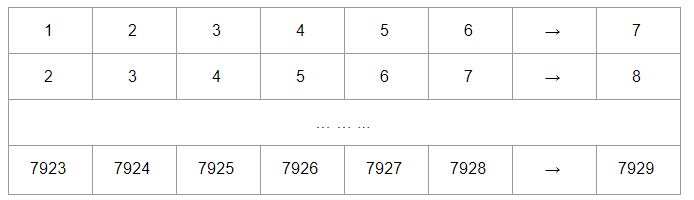
\includegraphics[scale=0.75]{dani.JPG}
    \begin{itemize}
        \item Svaka ćelija je skup atributa za jedan dan
        \item Jedan patern \texttt{input\_nodes} predstavlja 6 dana zaredom
        \texttt{concatenate((bias, (x\_train[day:(day+N)]).reshape(-1), output\_arr))}
    \end{itemize}
\end{frame}

%--------------------------------------------------------
\begin{frame}[fragile]{Izračunavanje h1,..., hm čvorova skrivenog sloja}
\begin{verbatim}
# Naivan pristup
h[0] = 1.0
for j in range(1, m+1):
    u = 0
    for i in range(0, n+1):
        u += input_nodes[i] * w_[i][j]
    h[j] = activation_f(u)
\end{verbatim}
\begin{figure}
    \centering
    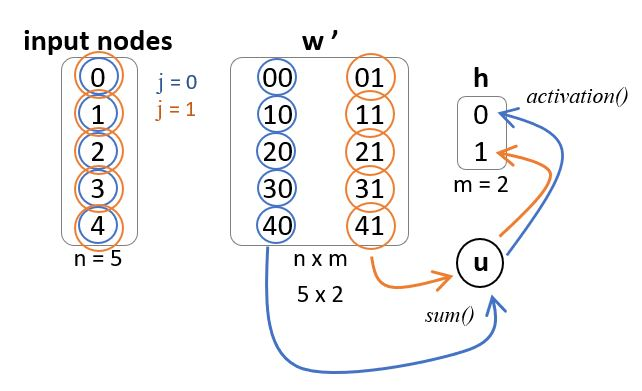
\includegraphics[scale=0.5]{naivno_izracunavanje_w_.JPG}
\end{figure}
\end{frame}

%--------------------------------------------------------
\begin{frame}[fragile]{Izračunavanje h1,..., hm čvorova skrivenog sloja}
\begin{verbatim}
# Poboljsan pristup
u = []
for i in w_.T:
    u += [activation_f(
            sum(multiply(i, input_nodes))
          )]
h = array(u)
h[0] = 1  # bias ostaje nepromenjen
\end{verbatim}
\begin{figure}
    \centering
    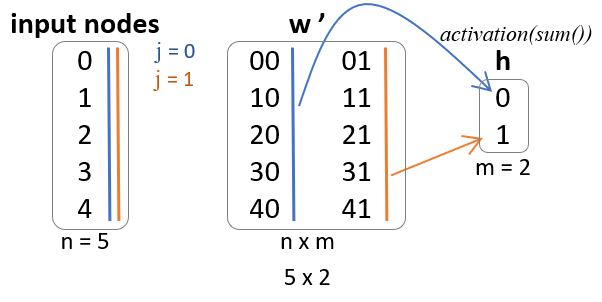
\includegraphics[scale=0.5]{izracunavanje_w_.JPG}
\end{figure}
\end{frame}

%--------------------------------------------------------
\begin{frame}[fragile]{Izračunavanje o1,...,op}
\begin{verbatim}
# Naivna implementacija
for k in range(1, p+1):
    u = 0
    for j in range(0, m+1):
        u += h[j] * w__[j][k]
    o[day] = activation_f(u)


# Poboljsana implementacija
o[day] = activation_f(sum(multiply(h, w__)))
output_arr = array([o[day]])
\end{verbatim}
\end{frame}

%--------------------------------------------------------
\begin{frame}{Računanje greške}
    Račun koji se može izdvojiti:\vspace{1cm}
    \\
    \texttt{error = (y\_train[day+N] - o[day]) * o[day] * (1.0 - o[day])}
    \vspace{1cm}
    \\
    Nadalje se samo koristi kao konstantna vrednost u izrazima.
\end{frame}


%--------------------------------------------------------
\begin{frame}[fragile]{Izračunavanje deltaH(j)}
Prednosti operacija sa vektorima:
\begin{verbatim}
# Naivna implementacija
for j in range(1, m+1):
    dh[j] = 0.0
    for k in range(1, p+1):
        dh[j] += w__[j][k] * error
        
# Poboljsana implementacija
dh = w__ * error
\end{verbatim}
\end{frame}


%--------------------------------------------------------
\begin{frame}[fragile]{Ažuriranje W'(ij) i deltaW'(ij)}
\begin{verbatim}
# Bukvalna interpretacija
for j in range(1,m+1):    
    for i in range(0,n+1): 
        dw_[i][j] = eta * input_nodes[i] * h[j] 
                    * (1 - h[j]) * dh[j] 
                    + alpha * dw_[i][j] 
        w_[i][j] += dw_[i][j]
\end{verbatim}
\end{frame}


%--------------------------------------------------------
\begin{frame}[fragile]{Ažuriranje W'(ij) i deltaW'(ij)}
\begin{verbatim}
# Naivna implementacija
for j in range(1, m+1):
    H = h[j] * (1 - h[j]) * dh[j]
    for i in range(0, n+1):
        dw_[i][j] = eta * input_nodes[i] * H 
                    + alpha * dw_[i][j]
        w_[i][j] += dw_[i][j]
\end{verbatim}
\begin{figure}
    \centering
    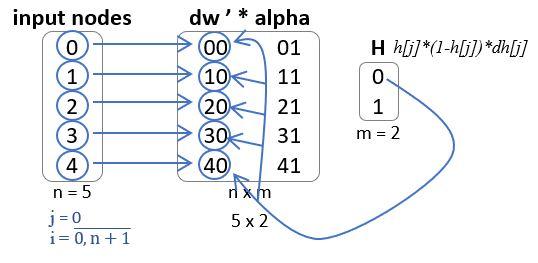
\includegraphics[scale=0.6]{azuriranje_w_.JPG}
\end{figure}
\end{frame}

%--------------------------------------------------------
\begin{frame}[fragile]{Ažuriranje W'(ij) i deltaW'(ij)}
\begin{verbatim}
# Poboljsana implementacija
H = h * (1-h) * dh * eta
dw_ *= alpha
for j in range(0, m):
    dw_.T[j] += (input_nodes * H[j])
w_ += dw_
\end{verbatim}
\begin{figure}
    \centering
    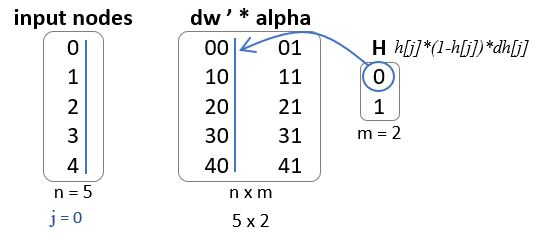
\includegraphics[scale=0.7]{poboljsano_azuriranje_w_.JPG}
\end{figure}
\end{frame}

%--------------------------------------------------------
\begin{frame}[fragile]{Ažuriranje W''(jk) i deltaW''(jk)}
    \begin{verbatim}
# Naivna implementacija
for k in range(1, p):
    for j in range(0, m):
        dw__[j][k] = eta * h[j] * error 
                    + alpha * dw__[j][k]
        w__[j][k] += dw__[j][k]
        

# Poboljsana implementacija
dw__ *= alpha
dw__ += (eta * h * error)
w__ += dw__
    \end{verbatim}
\end{frame}

%--------------------------------------------------------
\begin{frame}{Čuvanje modela i testiranje}
    \begin{itemize}
        \item Kroz epohe se beleži najbolji model.
        \item Moguće je učitati neki od postojećih modela kako bi se uštedelo na vremenu.
        \item Testiranje se sastoji od primene istih operacija korišćenjem postojećih težinskih matrica nad skupom za test.
    \end{itemize}
\end{frame}


\section{Primeri rezultata}
%--------------------------------------------------------
\begin{frame}[noframenumbering]
    Na narednim slajdovima prikazaćemo izlazne vrednosti programa kao i grafike koje smo dobili po epohama za različite vrednosti parametara.
    \\
    Grafici su radi bolje vidljivosti pravljeni za poslednjih 365 dana svoje epohe.
\end{frame}
%========================================================= 1
\begin{frame}{\small{Model \texttt{n = 54, m = 270, alpha = 0.5, eta = 0.3}}}
    \begin{center}
    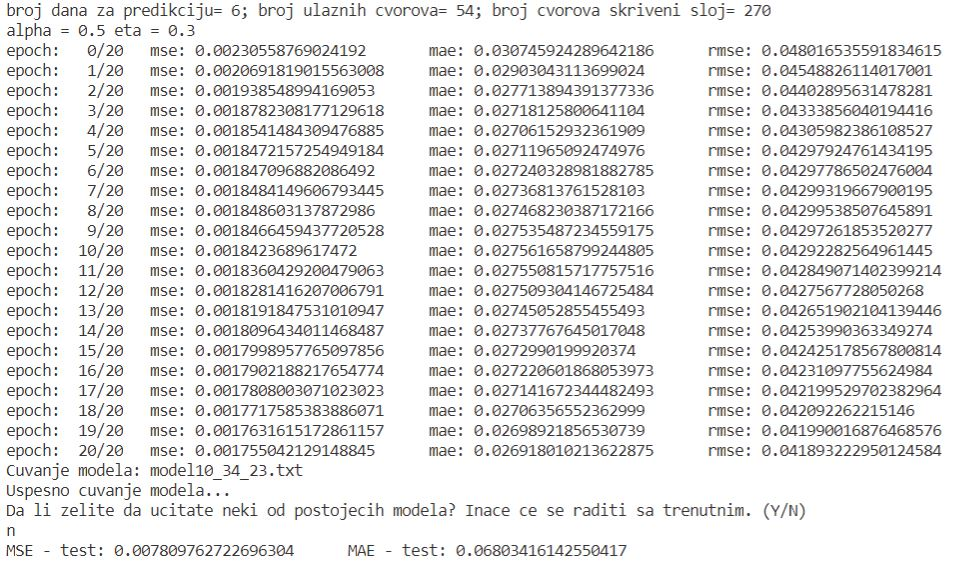
\includegraphics[scale=0.55]{output/output_example_program_10_34_23.JPG}
    \end{center}
\end{frame}

%--------------------------------------------------------
\begin{frame}{\small{Model \texttt{n = 54, m = 270, alpha = 0.5, eta = 0.3}}}
    \begin{figure}
    \centering
    \subfigure{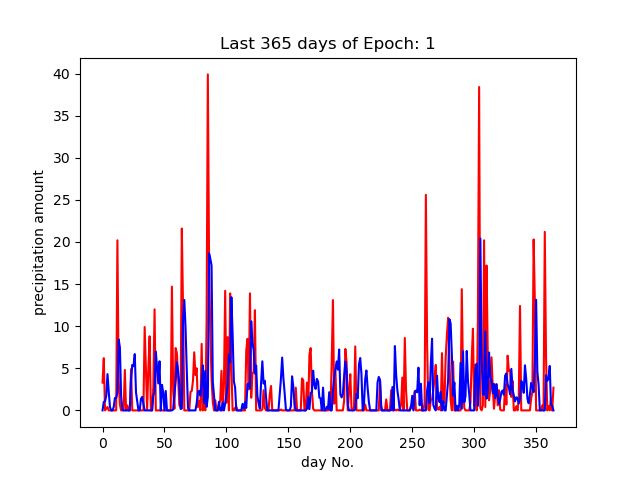
\includegraphics[width=0.45\linewidth]{plots/plot_epoch_1_time_10_34_23.png}} 
    \subfigure{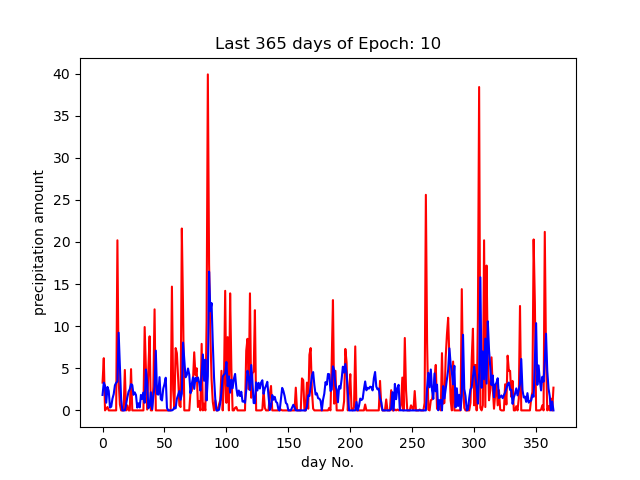
\includegraphics[width=0.45\linewidth]{plots/plot_epoch_10_time_10_34_23.png}} 
    \subfigure{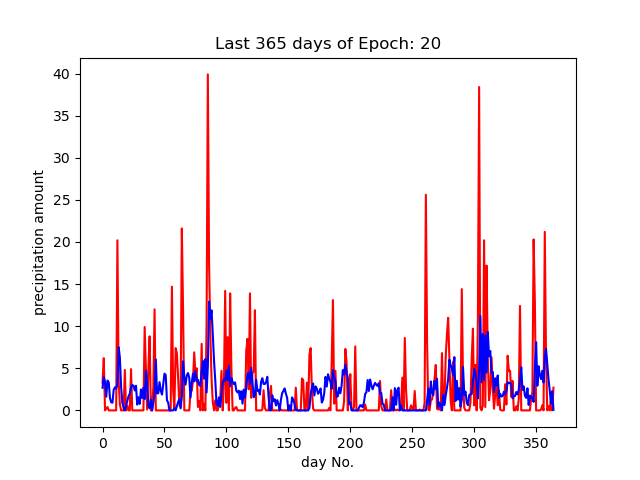
\includegraphics[width=0.45\linewidth]{plots/plot_epoch_20_time_10_34_23.png}}
    \subfigure{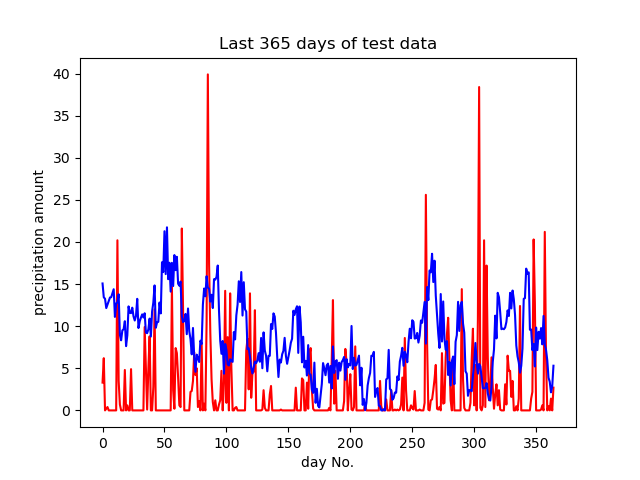
\includegraphics[width=0.45\linewidth]{plots/plot_test_model-model10_34_23-time_10_34_23.png}}
\end{figure}
\end{frame}

% ==================================================== 2

\begin{frame}{\small{Model \texttt{n = 54, m = 270, alpha = 0.2, eta = 0.3}}}
    \begin{center}
    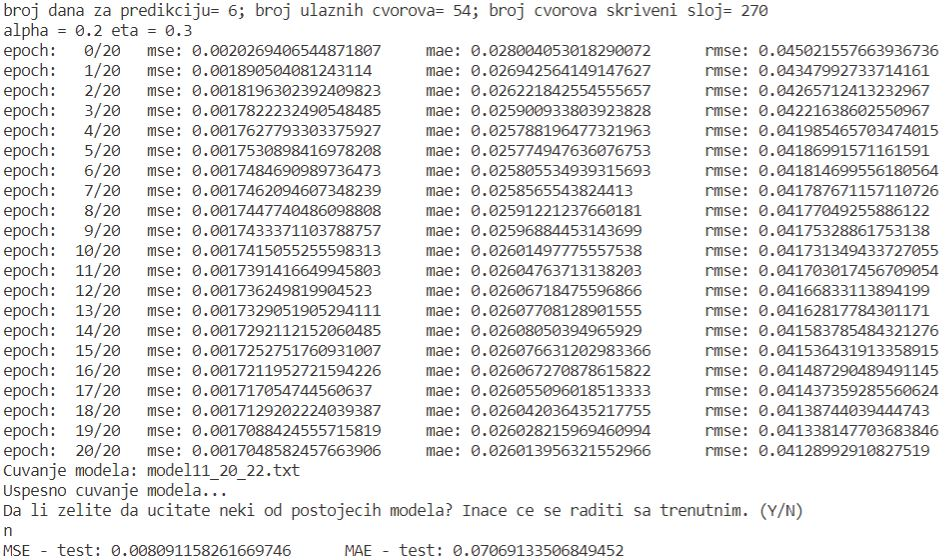
\includegraphics[scale=0.55]{output/output_example_program_11_20_22.JPG}
    \end{center}
\end{frame}

%--------------------------------------------------------
\begin{frame}{\small{Model \texttt{n = 54, m = 270, alpha = 0.2, eta = 0.3}}}
    \begin{figure}
    \centering
    \subfigure{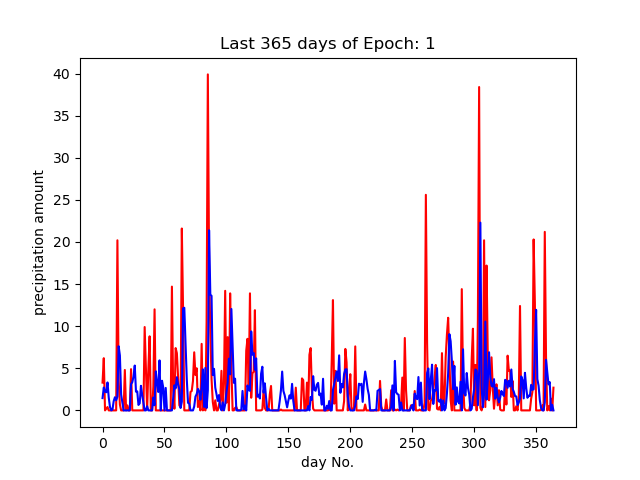
\includegraphics[width=0.45\textwidth]{plots/plot_epoch_1_time_11_20_22.png}} 
    \subfigure{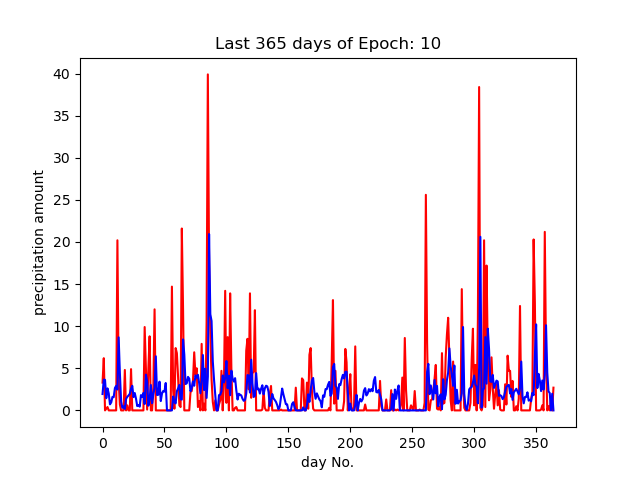
\includegraphics[width=0.45\textwidth]{plots/plot_epoch_10_time_11_20_22.png}} 
    \subfigure{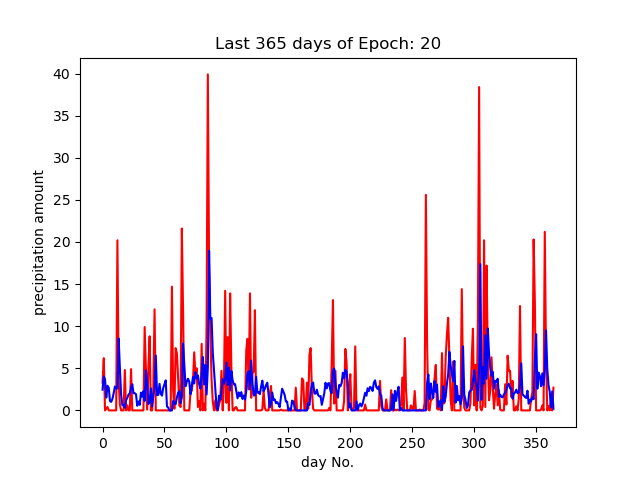
\includegraphics[width=0.45\textwidth]{plots/plot_epoch_20_time_11_20_22.png}}
    \subfigure{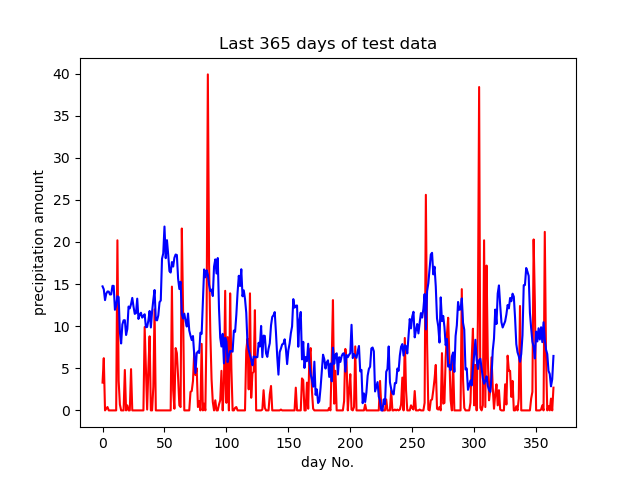
\includegraphics[width=0.45\textwidth]{plots/plot_test_model-model11_20_22-time_11_20_22.png}}
\end{figure}
\end{frame}

% ==================================================== 3

\begin{frame}{\small{Model \texttt{n = 54, m = 108, alpha = 0.2, eta = 0.3}}}
    \begin{center}
    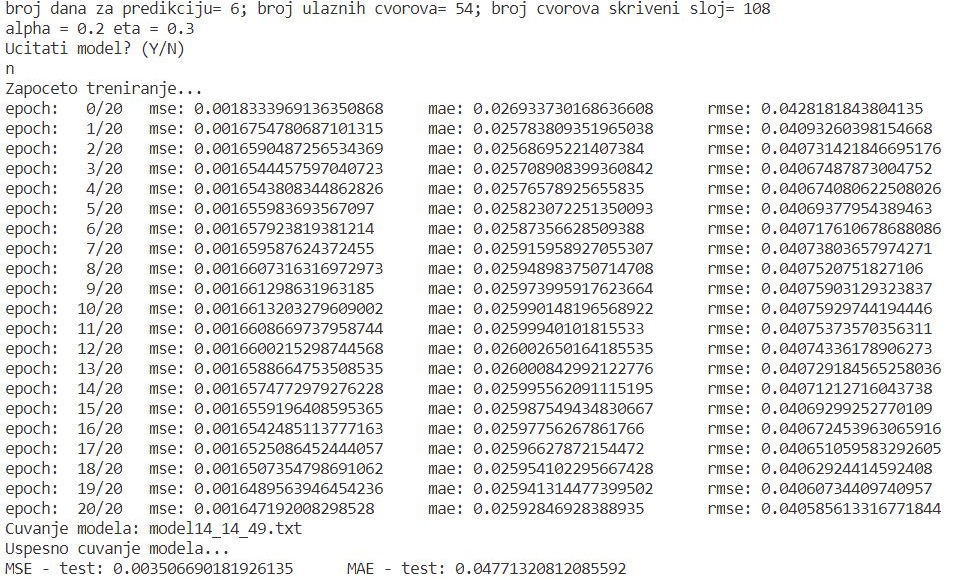
\includegraphics[scale=0.55]{output/output_example_program_14_14_49.JPG}
    \end{center}
\end{frame}

%--------------------------------------------------------
\begin{frame}{\small{Model \texttt{n = 54, m = 108, alpha = 0.2, eta = 0.3}}}
    \begin{figure}
    \centering
    \subfigure{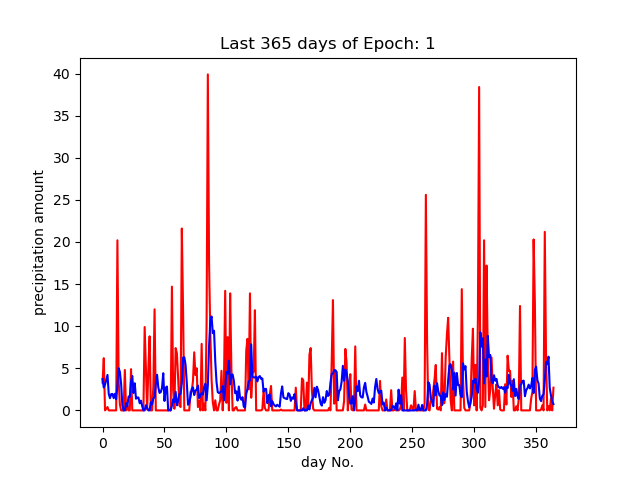
\includegraphics[width=0.45\textwidth]{plots/plot_epoch_1_time_14_14_49.png}} 
    \subfigure{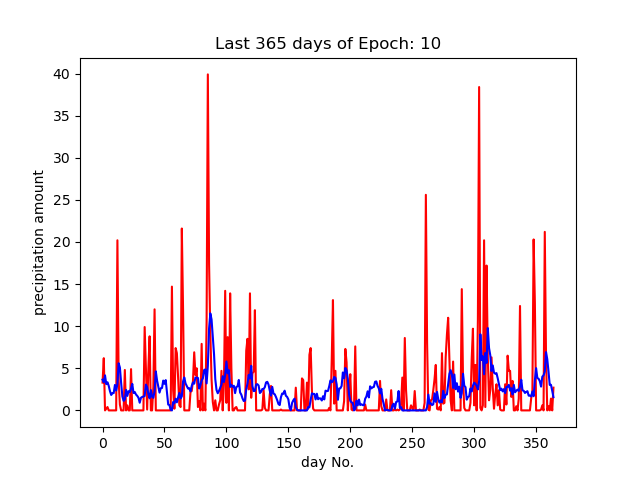
\includegraphics[width=0.45\textwidth]{plots/plot_epoch_10_time_14_14_49.png}} 
    \subfigure{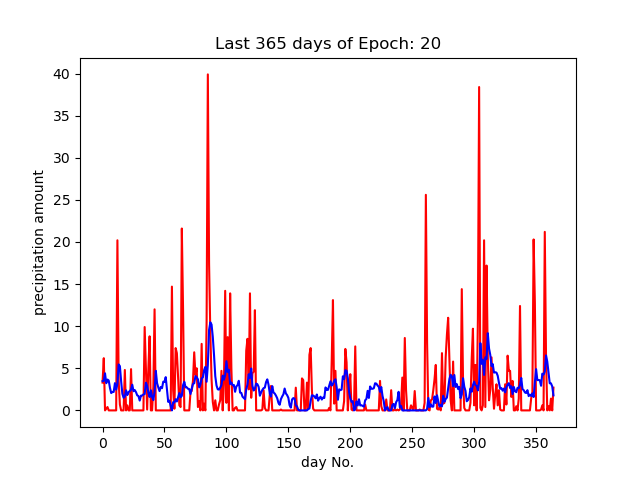
\includegraphics[width=0.45\textwidth]{plots/plot_epoch_20_time_14_14_49.png}}
    \subfigure{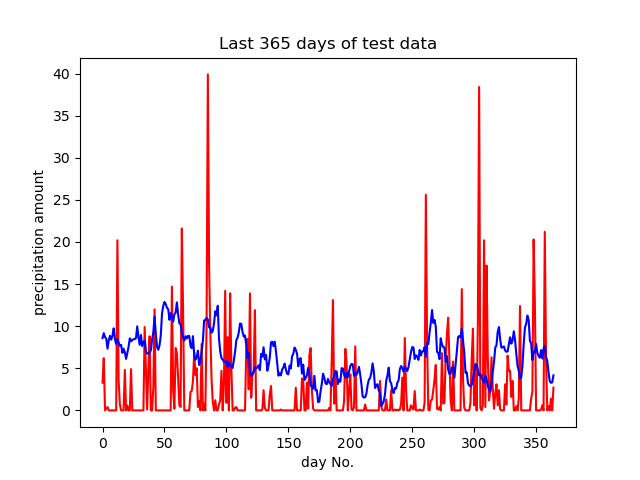
\includegraphics[width=0.45\textwidth]{plots/plot_test_model-model14_14_49-time_14_14_49.png}}
\end{figure}
\end{frame}

% ==================================================== 4

\begin{frame}{\small{{Model \texttt{n = 54, m = 108, alpha = 0.9, eta = 0.5}}}}
    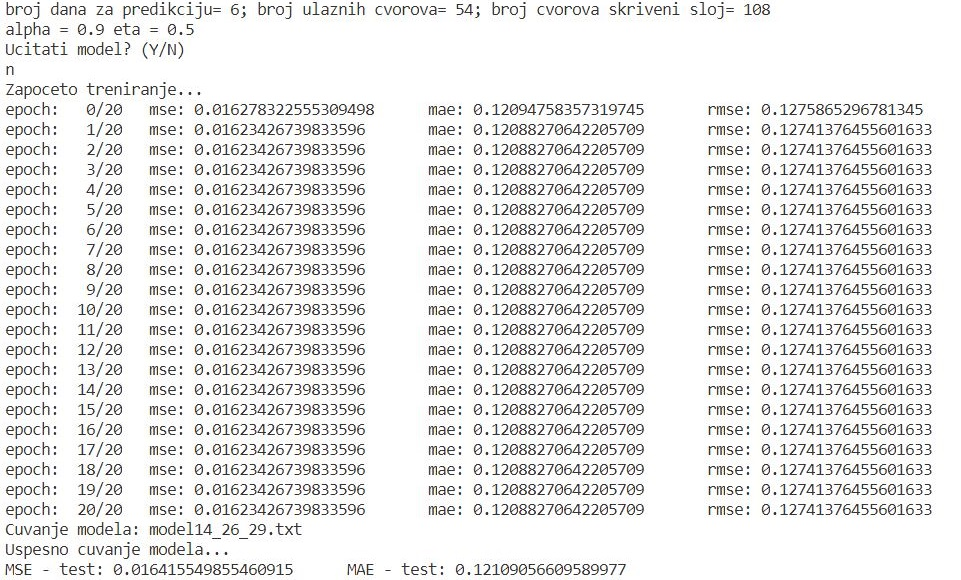
\includegraphics[scale=0.55]{output/output_example_program_14_26_29.JPG}
\end{frame}

%--------------------------------------------------------
\begin{frame}{\small{{Model \texttt{n = 54, m = 108, alpha = 0.9, eta = 0.5}}}}
    \begin{figure}
    \centering
    \subfigure{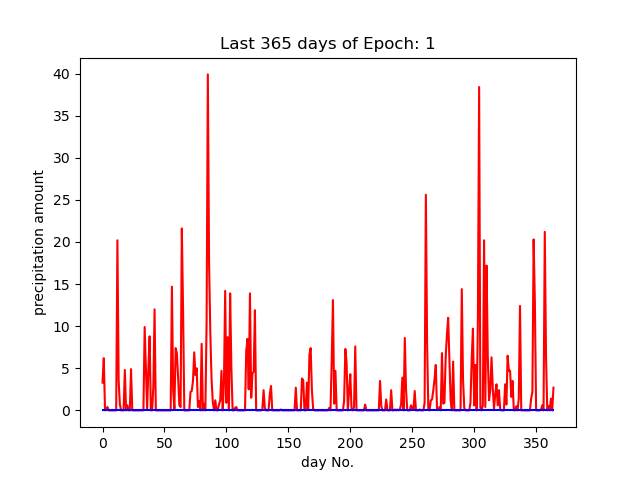
\includegraphics[width=0.45\textwidth]{plots/plot_epoch_1_time_14_26_29.png}} 
    \subfigure{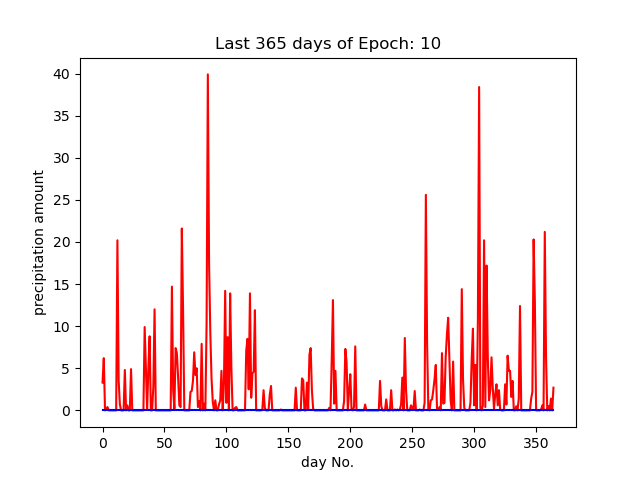
\includegraphics[width=0.45\textwidth]{plots/plot_epoch_10_time_14_26_29.png}} 
    \subfigure{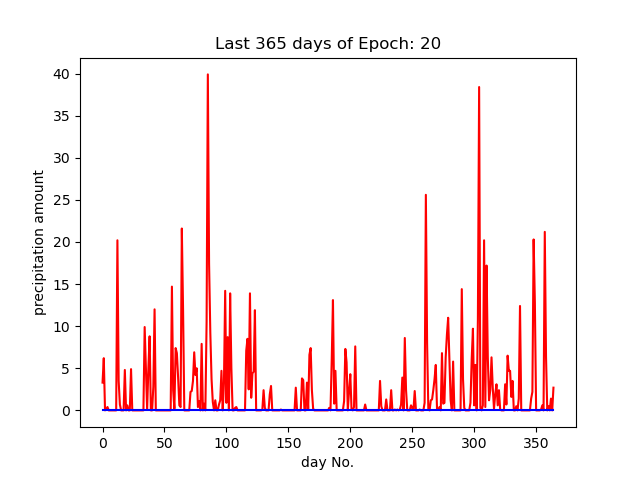
\includegraphics[width=0.45\textwidth]{plots/plot_epoch_20_time_14_26_29.png}}
    \subfigure{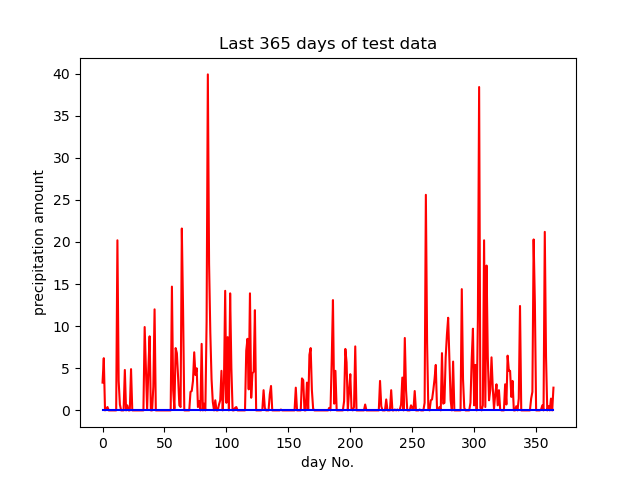
\includegraphics[width=0.45\textwidth]{plots/plot_test_model-model14_26_29-time_14_26_29.png}}
\end{figure}
\end{frame}

% ==================================================== 5

\begin{frame}{\small{{Model \texttt{n = 54, m = 216, alpha = 0.2, eta = 0.3}}}}
    \begin{center}
    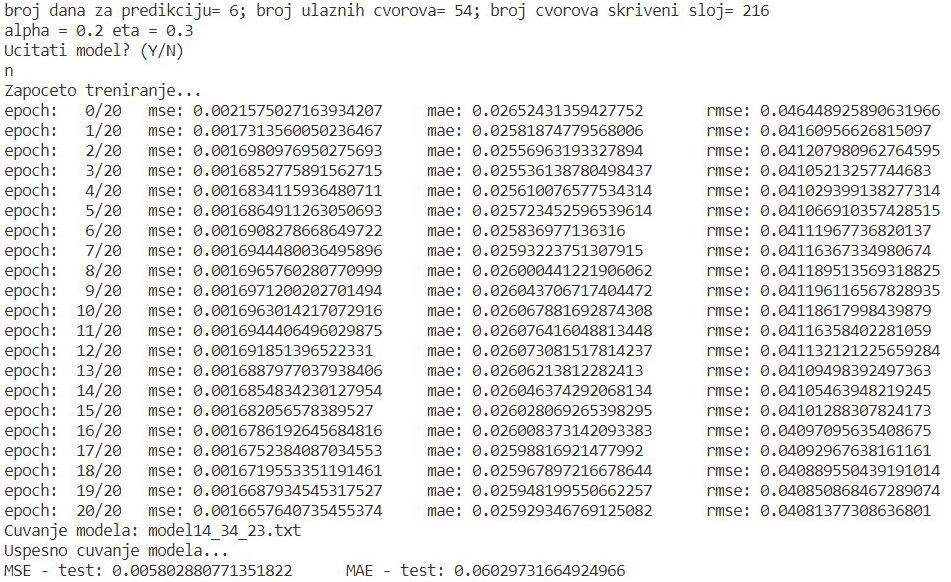
\includegraphics[scale=0.55]{output/output_example_program_14_34_23.JPG}
    \end{center}
\end{frame}

%--------------------------------------------------------
\begin{frame}{\small{{Model \texttt{n = 54, m = 216, alpha = 0.2, eta = 0.3}}}}
    \begin{figure}
    \centering
    \subfigure{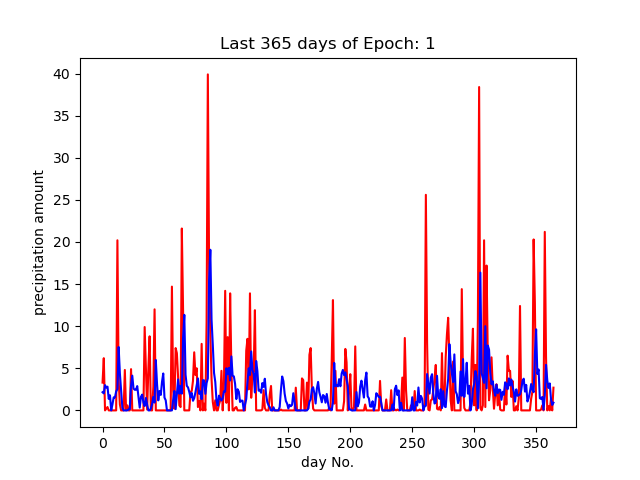
\includegraphics[width=0.45\textwidth]{plots/plot_epoch_1_time_14_34_23.png}} 
    \subfigure{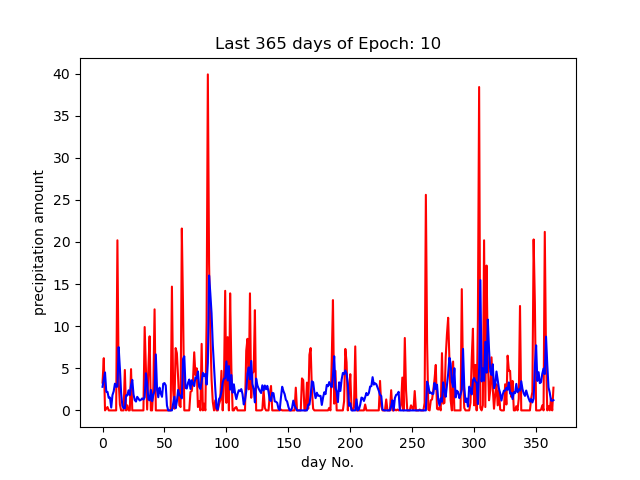
\includegraphics[width=0.45\textwidth]{plots/plot_epoch_10_time_14_34_23.png}} 
    \subfigure{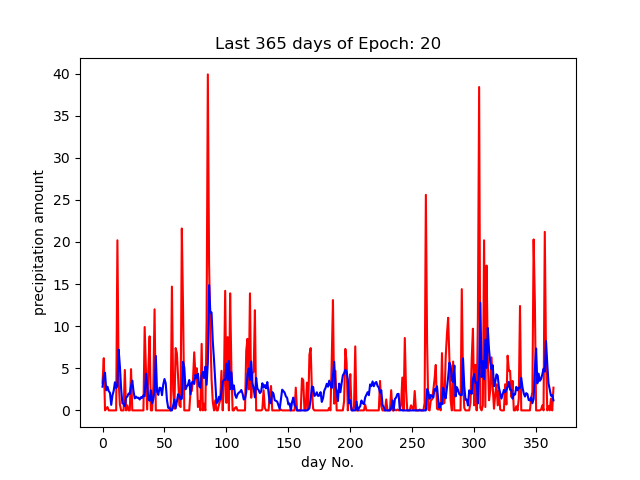
\includegraphics[width=0.45\textwidth]{plots/plot_epoch_20_time_14_34_23.png}}
    \subfigure{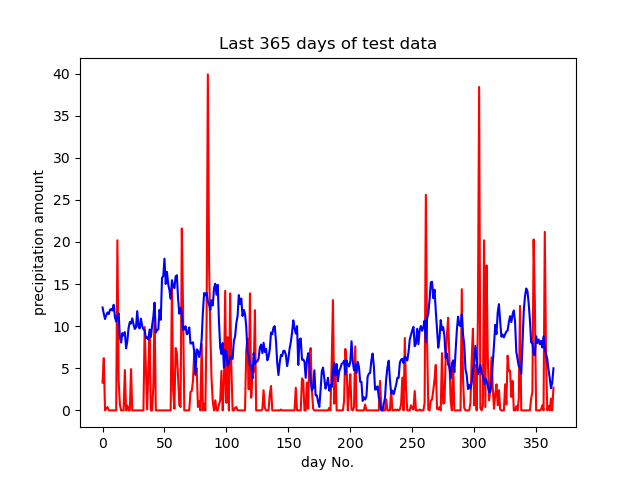
\includegraphics[width=0.45\textwidth]{plots/plot_test_model-model14_34_23-time_14_34_23.png}}
\end{figure}
\end{frame}

\section{Zaključak}

%--------------------------------------------------------
% \appendix

\begin{frame}{References}
    \nocite{*} % Display all references regardless of if they were cited
	\bibliography{seminarski.bib}
	\bibliographystyle{plain}
\end{frame}

\end{document}